%! Author = lazza
%! Date = 03/05/2022

\section{Dynamic Scheduling}\label{sec:dynamic-scheduling}
The hardware reorders the instruction execution to reduce pipeline stalls while maintaining data flow and exception behavior.

\paragraph{Main advantages}
\begin{itemize}
    \item[] It enables handling some cases where dependencies are unknown at compile time
    \item[] It simplifies the compiler complexity
    \item[] It allows compiled code to run efficiently on a different pipeline.
\end{itemize}

\paragraph{Costs} Advantages are gained at a cost:
\begin{itemize}
    \item[] A significant increase in hardware complexity
    \item[] Increased power consumption
    \item[] Could generate imprecise exception
\end{itemize}

\paragraph{In-order Issue}
Instructions are fetched and issued in program order (in-order-issue).
The execution begins as soon as operands are available, possibly, out of order execution.\\
\textbf{Note:} possible even with pipelined scalar architectures.

\paragraph{Out-of-order Execution}
Out-of order execution introduces possibility of WAR, WAW data hazards.
It implies out-of-order completion unless there is a re-order buffer to get in-order completion.

\paragraph{Example}
\begin{center}
    \begin{verbatim}
        DIVD FO,  F2, F4
        ADDD F10, F0, F8
        SUBD F12, F8, F14
    \end{verbatim}
    \textrightarrow RAW on F0, causes the \verb|SUBD| to stall without dynamic scheduling.

\end{center}

\textbf{Note:} As mentioned before, here we are talking strictly about the hardware, there could be software pipelining.

\

\subsection{Scoreboard}\label{subsec:scoreboard}
Suppose a data structure keeps track of all the instructions in all the functional units.
The following checks need to be made before the Issue stage can dispatch an instruction:
\begin{itemize}
    \item is the required function available?
    \item is the input data available? (RAW?)
    \item is it safe to write the destination? (WAR? WAW?)
\end{itemize}


\paragraph{Data structure} The instruction \textit{i} at the Issue stage consults this table
\begin{description}
    \item[FU available?]
check the busy column
    \item[RAW?]
search the dest column for i’s sources
    \item[WAR?]
search the source columns for i’s destination
    \item[WAW?]
search the dest column for i’s destination
\end{description}

\begin{table}[h]
    \centering
    \begin{tabular}{c|c|cccc}
        \toprule
        \textbf{Name} & \textbf{Busy} & \textbf{Op} & \textbf{Dest} & \textbf{Src1} & \textbf{Src2} \\
        \midrule
        Int &  &  &  &  &  \\
        Mem &  &  &  &  &  \\
        \midrule
        Add1 &  &  &  &  &  \\
        Add2 &  &  &  &  &  \\
        Add3 &  &  &  &  &  \\
        \midrule
        Mult1 &  &  &  &  &  \\
        Mult2 &  &  &  &  &  \\
        \midrule
        Div &  &  &  &  &  \\
        \bottomrule
    \end{tabular}
    \caption{Example of data structure for correct issues}
    \label{tab:scoreboard-data-structure}
\end{table}

\paragraph{CDC6600 Scoreboard}
\paragraph{In-order issue} Instructions dispatched in-order to functional units provided no structural hazard or WAW:
\begin{itemize}
    \item stall on structural hazard, no functional units available
    \item only one pending write to any register
\end{itemize}

\paragraph{Out-of-order read \& execution} Instructions wait for input operands in case of RAW hazards.
Once they read operands can execute out-of-order.

\paragraph{Out-of-order write} Instructions wait for output register to be read by preceding instructions in case
of WAR hazard, the result is held in functional unit until register is free, that is right after the register causing
the hazard is read.

\paragraph{Centralized hazard management} Every instruction goes through scoreboard:
\begin{itemize}
    \item it determines when the instruction can \textbf{read} its operands and \textbf{begin execution}
    \item it monitors changes in hardware and decides when a stalled instruction can \textbf{resume execution}
    \item it controls then instruction can \textbf{write} results
\end{itemize}

\subsubsection{Scoreboard Pipeline}\label{subsubsec:scoreboard-pipeline}
New pipeline ID stage split in two parts:

\begin{table}[h]
    \centering
    \begin{tabular}{|c|c|c|}
        \toprule
        \textbf{ID} & \textbf{EX} & \textbf{WB} \\
        \midrule
        Issue | Read Regs & Execution & Write \\
        \bottomrule
    \end{tabular}
    \caption{Scoreboard Pipeline}
    \label{tab:scoreboard-pipeline}
\end{table}

\begin{description}
    \item[Issue] Decode and check structural hazard.\\
    Instructions issued in program order (for hazard checking).

    If a functional unit for the instruction is free and no other
    active instruction has the same destination register (WAW),
    the scoreboard issues the instruction to the functional unit
    and updates its internal data structure.

    If a structural or a WAW hazard exists, then the instruction
    issue stalls, and no further instructions will issue until these
    hazards are cleared.

    \item[Read Operands] Wait until there are no data hazards, then read operands.\\
    A source operand is available if:
    \begin{itemize}[noitemsep]
        \item[-] no earlier issue active instructions will write it
        \item[-] a functional unit is writing its value in a register
    \end{itemize}
    When the source operands are available, the
    scoreboard tells the functional unit to proceed to read
    the operands from the registers and begin execution.
    RAW hazards are resolved dynamically in this step,
    and instructions may be sent into execution out-of-order.
    No forwarding of data in this model.

    \item[Execution] Operate on operands.\\
    The functional unit begins execution upon receiving operands.
    When the result is ready, it notifies the scoreboard that it has completed execution.
    FUs are characterized by:
    \begin{itemize}[noitemsep]
        \item[-] latency (the effective time used to complete one
        operation)
        \item[-] Initiation interval (the number of cycles that must
        elapse between issuing two operations to the same
        functional unit).
    \end{itemize}

    \item[Write result] Finish execution.\\
    Once the scoreboard is aware that the
    functional unit has completed execution, the
    scoreboard checks for WAR hazards: if none, it writes results.
    If there's a WAR, then it stalls the instruction.
    Assume we can overlap issue and write.
\end{description}

\paragraph{Scoreboard implications}
Solution for WAW:
    – Detect hazard and stall issue of new instruction until the other instruction completes.
No register renaming.
Need to have multiple instructions in execution
phase ---> Multiple execution units or pipelined
execution units.
Scoreboard keeps track of dependencies and
state of operations.

\paragraph{Example}
\begin{center}
    \begin{verbatim}
        DIVD  F0,  F2,  F4
        ADDD  F6,  F0,  F8
        SUBD  F8,  F8,  F14
        MULD  F6,  F10, F8
    \end{verbatim}
\end{center}
SUBD in the WB stage, waiting that ADDD reads F0 and F8 and MULD in the issue stage until ADDD writes F6. Cannot be
solved without register renaming.\\

\subsubsection{Scoreboard Structure}\label{subsubsec:scoreboard-structure}
\begin{description}
    \item[Instruction Status] Tells witch instruction is being executed.
    \item[FU Status] Indicates the state of the functional unit (FU):
    \begin{itemize}[noitemsep]
        \item[] Busy – Indicates whether the unit is busy or not
        \item[] Op - The operation to perform in the unit (+,-, etc.)
        \item[] Fi - Destination register
        \item[] Fj, Fk – Source register numbers
        \item[] Qj, Qk – Functional units producing source registers (RAW)
        \item[] Rj, Rk – Flags indicating when Fj, Fk are ready (WAR)
    \end{itemize}
    \item[Register Result Status] Indicates which functional unit will write each register.
Blank if no pending instructions will write that register.
\end{description}

\subsection{Tomasulo}\label{subsec:tomasulo}
\paragraph{Distributed management control} The control logic and the buffers are distributed with FUs (vs centralized in
scoreboard).

\subsubsection{Reservation Stations}
Operand buffers are called Reservation Stations.
Each instruction is an entry of a reservation station.
\begin{figure}[h]
    \centering
    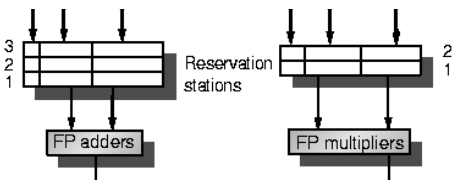
\includegraphics[scale = 0.4]{images/reservation-station}
    \caption{Reservation stations (RS)}
    \label{fig:reservation-stations}
\end{figure}
Components:
\begin{description}[style=multiline,leftmargin=2cm,font=\normalfont]
    \item[Tag] identifying the RS
    \item[OP] Operation to perform on the component.
    \item[Vj,Vk] Value of the source operands.
    \item[Qj,Qk] Pointers to RS that produce Vj,Vk. Zero value = Source op is already available in Vj or Vk.
    \item[Busy] Indicates RS Busy.
\end{description}
\textbf{Note:} Only one of V-field or Q-field is valid for each operand.\\

Reservation stations allow for:
\begin{itemize}
    \item[\textrightarrow] \underline{Register Renaming:} the operands of the RSs are replaced by values or pointers:
    \begin{itemize}
        \item avoid WAR and WAW hazards
        \item \# reservation stations > \# registers, make possible better optimization than a compiler
    \end{itemize}
    \item[\textrightarrow] \underline{Loop unrolling} in hardware: permit instruction issue to advance past integer
    control flow operations (thanks to register renaming)
    \item[\textrightarrow] \underline{Distribute management control}
\end{itemize}

\subsubsection{Common data bus}
Results are dispatched to other FUs through a Common Data Bus (CDB).
It offers a \textit{serialized} access to write back.
It provides values before they are saved into registers, that is data forwarding: it makes a point-to-point connection
between the FU providing the result and the FU(s) waiting for input.
The \verb|load| and \verb|store| operations are treated as FUs.

\begin{figure}
    \centering
    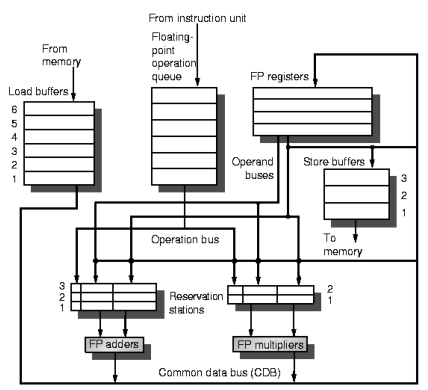
\includegraphics[scale = 0.5]{images/tomasulo-architecture}
    \caption{Tomasulo architecture}
    \label{fig:tomasulo-architecture}
\end{figure}

\subsubsection{Other Components}
The Register File and the Store Buffer have a \textit{value} (V) and a \textit{pointer}
(Q) field.\\
Q corresponds to the reservation station(s) producing the result to be stored in RF or store buffer.
If zero (or \verb|null|), there are no active instructions producing the result (RF or store buffer content has the
correct value).
\begin{table}[H]
    \centering
    \begin{tabular}{l|ll}
        \textbf{} & \textbf{V} & \textbf{Q} \\
        \midrule
        F0 &  &  \\
        \midrule
        F1 &  &  \\
        \midrule
        ... &  &  \\
        \bottomrule
    \end{tabular}
    \caption{Register File - RF}
    \label{tab:register-file}
\end{table}

Load and store buffers have an \textit{address} (A) field, and a \textit{busy} field.

\begin{table}[H]
    \centering
    \begin{tabular}{l|ll}
        \textbf{} & \textbf{busy} & \textbf{A} \\
        \midrule
        Load1 &  &  \\
        \midrule
        Load2 &  &  \\
        \bottomrule
    \end{tabular}
    \caption{Load buffer}
    \label{tab:load-buffer}
\end{table}

\begin{table}[H]
    \centering
    \begin{tabular}{l|lll}
        \textbf{} & \textbf{busy} & \textbf{A} & \textbf{Q}\\
        \midrule
        Store1 &  &  &\\
        \midrule
        Store2 &  &  &\\
        \bottomrule
    \end{tabular}
    \caption{Store buffer}
    \label{tab:store-buffer}
\end{table}

\textbf{Note:} The \textit{address} field holds info for memory address calculation for load/store.
Initially contains the instruction offset (immediate field), after address calculation stores the effective address.

\subsubsection{Tomasulo Stages}
\begin{description}
    \item[Issue] Get an instruction I from the queue.\\
    If it is an FP op check if a RS is empty (i.e., check for structural hazards).\\
    If it is a \verb|ld| or \verb|sd| check if the corresponding buffers have a free spot.

    \underline{Rename registers:}
    \begin{itemize}
        \item[\textrightarrow] WAR resolution\\
    If I writes Rx, read by an instruction K already issued, K
    knows already the value of Rx or knows what instruction
    will write it.
    So the RF can be linked to~I (with Q pointer).
        \item[\textrightarrow] WAW resolution\\
    Since we use in-order issue, the RF can be linked to~I
    \end{itemize}

    \item[Execution] When both operands are ready then execute.

    If not ready, watch the CDB for results: delay execution until operands are available, RAW
    hazards are avoided.\\
    \textbf{Note:} multiple instructions could become ready in the
    same clock cycle for the same FU, start execution only if there's a free FU\@.

    Load and stores, two-step process:
    \begin{itemize}[noitemsep]
        \item[\textbf{1.a-b}] compute effective address, place it in load or
        store buffer (in A field).
        \item[\textbf{2.a}] Loads in Load Buffer execute as soon as memory unit is
    available.
        \item[\textbf{2.b}] Stores in store buffer wait for the value pointed by Q before
    being sent to memory unit.
    \end{itemize}

    \item[Write] When result is available, write on Common Data Bus and from there into RF and into all RSs
    (including store buffers) waiting for this result then mark reservation stations available.\\
    \textbf{Note:} In the general case of concurrent writes, choose first the one that belongs to the critical path.
\end{description}


\subsubsection{Tomasulo in detail}
All writes occur in Write Result, simplifying
Tomasulo algorithm.

A Load and a Store can be done in different
order, provided they access different memory
locations.
Otherwise, a WAR (interchange load-store
sequence) or a RAW (interchange store-load
sequence) may result (WAW if two stores are
interchanged).
Loads can be reordered freely.\\
\textbf{Note:} registers are renamed but memory locations remain the same.

To detect such hazards: data memory
addresses associated with any earlier memory
operation must have been computed by the
CPU (i.e., address computation executed in
program order)

Load executed out of order with previous store:
assume address computed in program order.
When Load address has been computed, it
can be compared with A fields in active Store
buffers: in the case of a match, Load is not sent
to Load buffer until conflicting store completes.

Stores must check for matching addresses in
both Load and Store buffers (dynamic
disambiguation, alternative to static
disambiguation performed by the compiler)

Drawback: amount of hardware required.

Each RS must contain a fast associative buffer;
single CDB may limit performance.

\subsubsection{Tomasulo Drawbacks}
\begin{itemize}
    \item complexity
    \item large amount of hardware
    \item many associative store (CDB) at high speed
    \item performance limited by CDB
\end{itemize}
Multiple CDBs $\Longrightarrow$ more FU logic for parallel associative
stores.

\paragraph{Scoreboard vs Tomasulo}
\begin{itemize}
    \item[\textrightarrow] structural hazards in scoreboard
    \item[\textrightarrow] lack of forwarding in scoreboard
\end{itemize}
